
\pagebreak
\setcounter{secnumdepth}{0}
\appendix
\section{Appendix I}
\setcounter{secnumdepth}{0}
\large {\textbf{KL3M Data Gallery}}
\begin{figure}[h!]
\centering
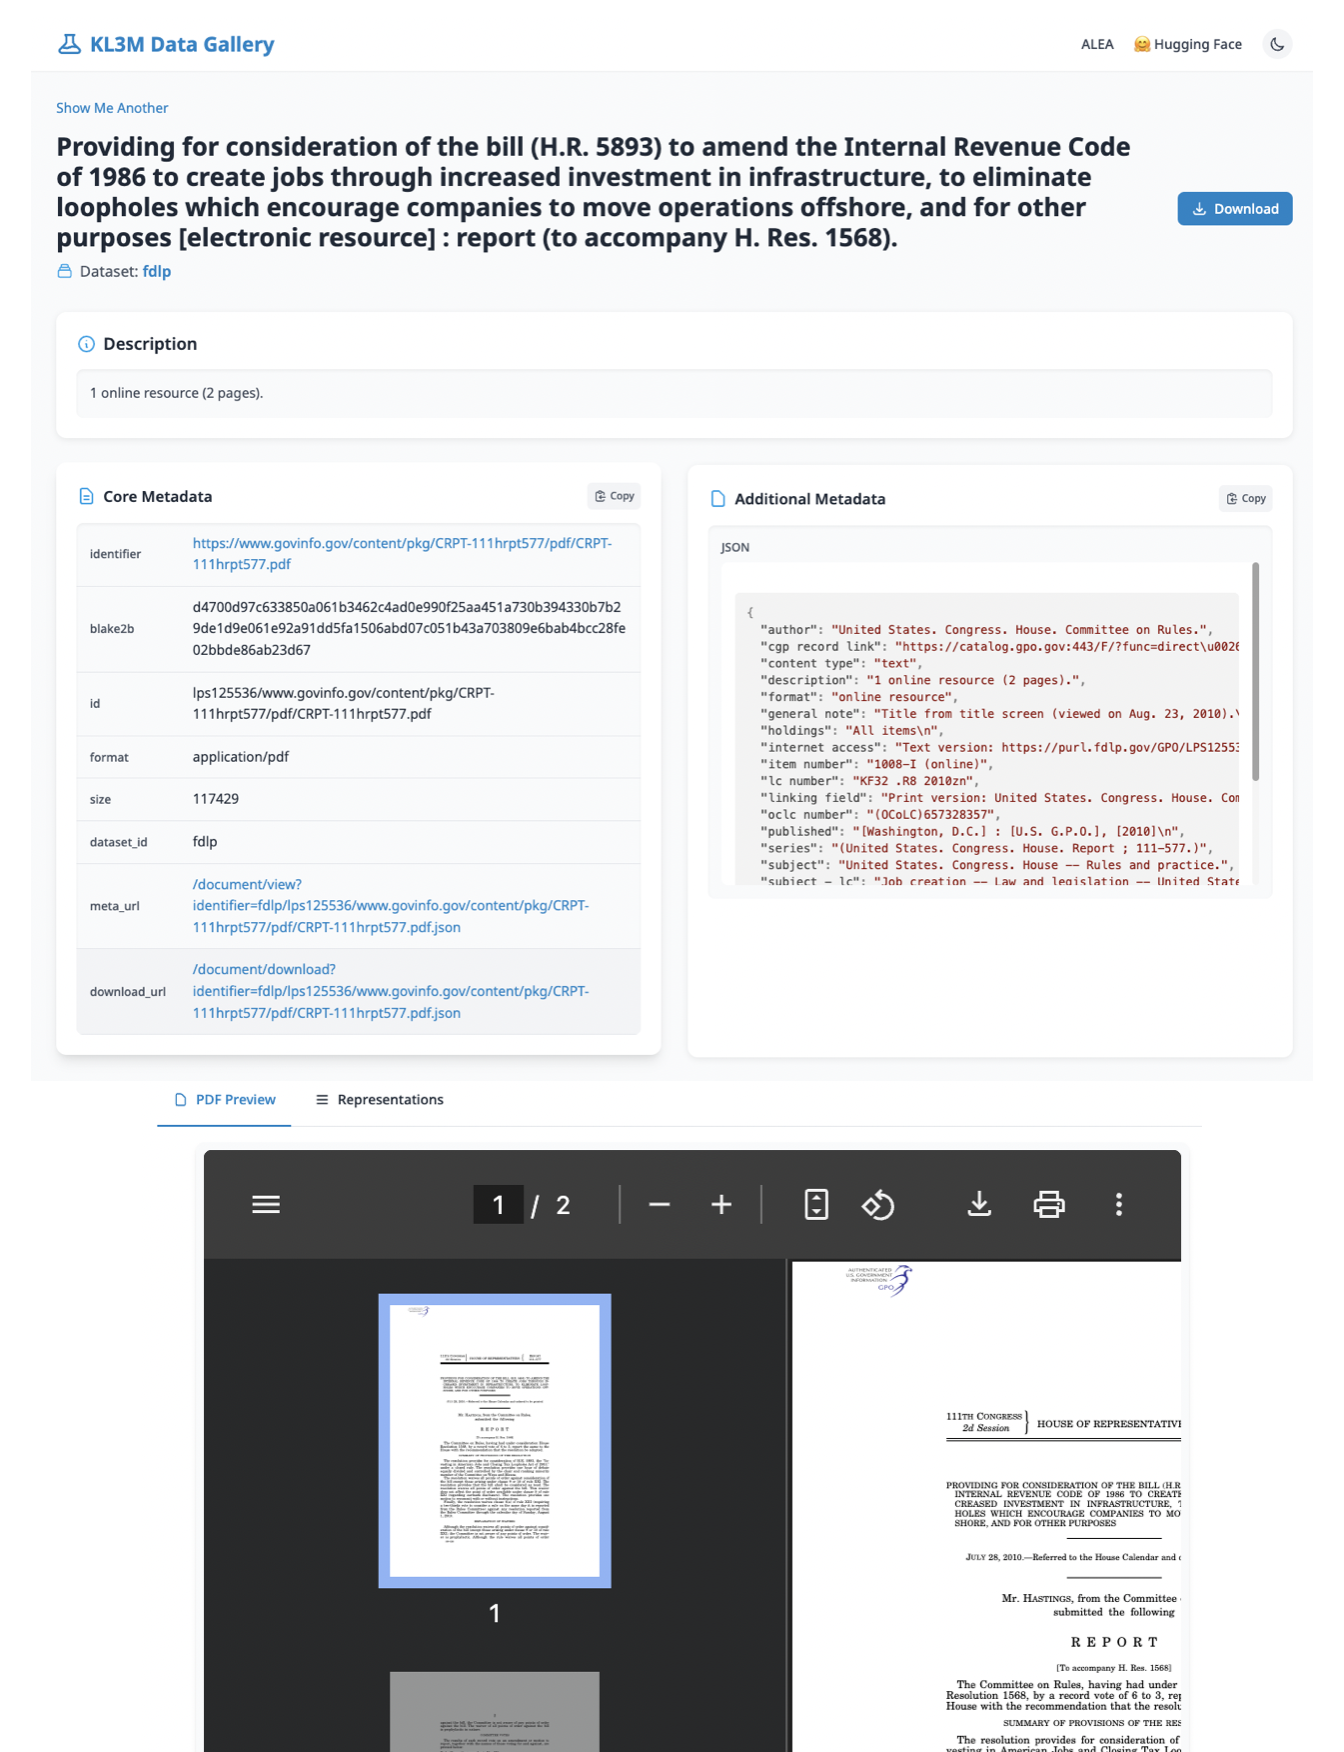
\includegraphics[width=120mm]{KL3MGallery.png}
\caption{\centering{KL3M Data Gallery - \url{https://gallery.kl3m.ai/}}}
\label{fig:method}
\end{figure}





\pagebreak
\section{\textbf{Appendix II}}
\setcounter{secnumdepth}{0}
\large {\textbf{KL3M Components Detailed Description}}
\begin{table}[h!]
\scriptsize
\begin{longtable}{ p{3cm} p{9cm} }
\textbf{KL3M Component}
& \textbf{Description}
\\\midrule
Securities \& Exchange Commission Filings & The U.S. Securities and Exchange Commission (SEC) is an independent agency of the federal government of the United States. As part of its role, the SEC requires public companies and other regulated entities to submit numerous filings and disclosures, which with limited exceptions (such as redacted information) are in the public domain. The KL3M dataset includes the following data subsets from the SEC: Public agreements, 10-K, 10-Q, 8-K, 6-K filings (foreign and domestic), Various S Filings, 6-K, 20-F, 40-F and associated exhibits and addenda.
\\
 \\\hline
 \\
Congressional Documents
& The Congressional Documents Collection is a collection of various materials ordered to be printed by both the U.S. House and Senate. It is comprised of House Documents, Senate Documents, and Senate Treaty Documents. The House and Senate Documents contain various kinds of materials ordered to be printed by both chambers of Congress, including executive reports from agencies and departments. The Senate Treaty Documents contain treaty text as it has been submitted by the Senate for presidential ratification.
\\
 \\\hline
  \\
Congressional Bills &
This component includes legislative proposals within the United States Congress from the House of Representatives and Senate. This includes the entire life cycle of bills, from initial introduction to final published bills.
\\
 \\\hline
  \\
Code of Federal Regulations &
The Electronic Code of Federal Regulations (eCFR) is an editorial compilation of CFR material and amendments published in the daily Federal Register. The eCFR is continuously updated, but is not the official legal edition of the CFR.
\\
 \\\hline
  \\
Electronic Code of Federal Regulations &
The Electronic Code of Federal Regulations (eCFR) is an editorial compilation of CFR material and amendments published in the daily Federal Register. The eCFR is continuously updated, but is not the official legal edition of the CFR.
\\
 \\\hline
  \\
Federal Depository
Library Program &
The Federal Depository Library Program (FDLP) provides a digitized record of the official documents published by the U.S. Government Publishing Office (GPO), GPO’s Superintendent of Documents, and other Federal agency publishers related to the FDLP.
\\
 \\\hline
  \\
Federal Register &
The Federal Register is the official daily publication for the following materials of the United States Federal Government: Presidential Documents, Executive Orders, proposed, interim, and final rules and regulations, and notices by Federal Agencies, as well as notices of hearings, decisions, investigations, and committee meetings. The National Archives and Records Administration is responsible for publishing the Federal Register.
\\
 \\\hline
  \\
Federal Judicial Center &
The Federal Judicial Center serves as the education and research agency for the U.S. federal courts. The KL3M dataset contains material published by the Federal Judicial Center, including research reports, monographs on substantive legal subjects, manuals, and reference guides.
\\
 \\\hline
    \end{longtable}

\end{table}
\pagebreak

\begin{table}[h]
\scriptsize
\begin{longtable}{ p{3cm} p{9cm} }
\textbf{KL3M Component}
& \textbf{Description}
\\\midrule
\\
CIA World Factbook &
The World Factbook, developed by the U.S. Central Intelligence Agency (CIA), provides basic intelligence on the history, people, government, economy, energy, geography, environment, communications, transportation, military, terrorism, and transnational issues for 265 world entities.
\\
 \\\hline
  \\
Congressional Research Service
& The Congressional Research Service (CRS) is a U.S. federal legislative branch agency that provides research services exclusively to congressional committees and Members of Congress. CRS reports, which are available to the public, cover a broad range of topics and are intended to reflect objective, nonpartisan research and analysis.
\\
 \\\hline
  \\
United States Government Manual &
The U.S. Government Manual is a regularly updated special edition of the Federal Register. Its contents include leadership tables and descriptions of agency activities and programs of the executive, judicial, and legislative branches of Federal U.S. Government, as well as those of quasi-official agencies and international organizations in which the United States is a participating member.
\\
 \\\hline
  \\
Library of Congress - Country Profiles &
This collection of nearly 50 country profiles of foreign nations provides brief, summarized information on each country’s historical background, geography, society, economy, transportation and telecommunications, government and politics, and national security. This series of profiles is a subset of the Country Studies Program, formerly the Army Area Handbook Program. The collection was written between 2004 and 2008 and has not been updated since then.
\\
 \\\hline
  \\
Statutes at Large &
The United States Statutes at Large is the permanent collection of all laws and resolutions enacted during each session of Congress. The Statutes at Large is prepared and published by the Office of the Federal Register (OFR). The printed edition of the Statutes at Large is legal evidence of the laws, concurrent resolutions, proclamations by the President, and proposed and ratified amendments to the Constitution.  \\
 \\\hline
  \\
Regulatory Submissions &
Any member of the public may submit comments on U.S. federal regulation through the website regulations.gov. The KL3M dataset contains the documents submitted as attachments to public comments. \\
 \\\hline
  \\
United States Code &
The United States Code is a consolidation and codification by subject matter of the general and permanent federal laws of the United States. It is prepared by the Office of the Law Revision Counsel of the United States House of Representatives.
\\
 \\\hline
  \\
Court Documents - Opinions &
U.S. federal and state court opinions are written explanations from judges that explain their decision and the facts and legal reasoning supporting it. The KL3M dataset contains court opinions obtained from two sources: PACER and CourtListener.  \\
 \\\hline
    \end{longtable}

\end{table}
\pagebreak


\begin{table}[!ht]
\scriptsize
\begin{longtable}{ p{3cm} p{9cm} }
\textbf{KL3M Component}
& \textbf{Description}
\\\midrule
\\
Court Documents Motions, Orders, etc. & Non-opinion court materials, such as motions, orders, and depositions were obtained through PACER. The non-opinions included in the KL3M dataset reflect content from federal courts only.   \\\\
 \\\hline
 \\
\textcolor{red}{\textbf{Court Documents - Dockets}}
&
\textcolor{black}{}\textbf{FILL THIS HERE}

\\
 \\\hline
  \\
Black's Law Dictionary, 2nd Edition &
The second edition of ``A Law Dictionary'' by Henry Campbell Black, commonly known as "Black's Law Dictionary" is a legal dictionary published in 1910 that contains definitions of the terms and phrases of both ancient and modern American and English jurisprudence \\\\
 \\\hline  \\
U.S. Federal Government Websites &
The KL3M dataset includes filtered content from websites of Federal agencies and departments of the United States. The content was filtered to limit inclusion to only that which is in the public domain.  \\
 \\\hline
 \\
US Patent Grant Full Text Data &
The United States Patent and Trademark Office (USPTO) publishes the full text, images/drawings, and complex work units (tables, mathematical expressions, chemical structures, and genetic sequence data) of each patent that is granted. The KL3M dataset only contains the full text of granted patents.
  \\
 \\\hline
 \\
 Official Journal of the European Union &
The Official Journal of the European Union is the official publication for EU legal acts, other acts and official information from EU institutions, bodies, offices and agencies. \\
 \\\hline
    \end{longtable}

\end{table}
